\documentclass[12pt,letterpaper]{article}
\usepackage[UTF8]{ctex}
\usepackage{fullpage}
\usepackage[top=2cm, bottom=4.5cm, left=2.5cm, right=2.5cm]{geometry}
\usepackage{amsmath,amsthm,amsfonts,amssymb,amscd}
\usepackage{lastpage}
\usepackage{enumerate}
\usepackage{fancyhdr}
\usepackage{mathrsfs}
\usepackage{xcolor}
\usepackage{graphicx}
\usepackage{listings}
\usepackage{hyperref}
\usepackage{dot2texi}
\usepackage{tikz}
\usepackage{float}
\usepackage[pdf]{graphviz}
\usetikzlibrary{automata,shapes,arrows} 

\hypersetup{%
  colorlinks=true,
  linkcolor=blue,
  linkbordercolor={0 0 1}
}
 
\renewcommand\lstlistingname{Algorithm}
\renewcommand\lstlistlistingname{Algorithms}
\def\lstlistingautorefname{Alg.}

\lstdefinestyle{Matlab}{
    language        = matlab,
    frame           = lines, 
    basicstyle      = \footnotesize,
    keywordstyle    = \color{blue},
    stringstyle     = \color{green},
    commentstyle    = \color{red}\ttfamily
}
\setlength{\parindent}{0.0in}
\setlength{\parskip}{0.05in}

% Edit these as appropriate
\newcommand\course{课程名称}
\newcommand\hwnumber{1}                  % <-- homework number
\newcommand\name{唐一早}                 % <-- Name
\newcommand\ID{2100012613}           % <-- ID

\pagestyle{fancyplain}
\headheight 35pt
\lhead{\name\\\ID}                 
\chead{\textbf{\Large Homework \hwnumber}}
\rhead{\course \\ \today}
\lfoot{}
\cfoot{}
\rfoot{\small\thepage}
\headsep 1.5em



\title{Log-Linear Lab Report}
\begin{document}

\maketitle

\section{项目使用方法}

项目主体包括三个文件 get\_feature.py , training.py , evaluation.py 。其中 get\_feature.py 会从训练集中获取特征并将特征保存在 ./features\&model/feature.txt 中。 training.py 会使用得到的特征进行预训练,并控制特征数量,然后使用预训练过的模型和削减过的特征进行训练,得到的特征和模型数据保存在 ./features\&model/real\_feature.txt 和 ./features\&model/model.txt 中。在训练集上得到的 score 保存在 ./result/acc.txt 中。 evaluation.py 会对得到的模型进行测试,测试结果保存在 ./result/acc.txt 中

您可以使用 run.sh 运行我的项目或者修改部分参数。如果您只想对模型进行测试您可以在命令行中运行

./run.sh 1 

如果您想修改某些模型参数并重新训练您可以在命令行中运行

./run.sh 2 

ps:目前参数的训练时常可能达数十分钟。

\section{训练集预处理}

get\_feature.py 中的 sentence\_process() 函数对每个句子做预处理,把标题和句子拼接,大写转化为小写,把所有数字用 'DIGITAL' 代替。

\section{特征提取方法}

我在 get\_feature.py 中对训练集中的数据先根据四个分类对每个词计算 TF 值并计算 idf 值。我首先根据 tf-idf 大小从高到低选取 unigram-feature , World 分类中前10个 feature 单词结果如下

'the', 'in', 'to', 'a', 'of', 'DIGITAL', 's', 'and', 'on', 'for'

结果很差,因为 tf-idf 值适用于对较短的句子文章提取特征词,难以用在一个分类的所有数据中,这样会导致出现频率特别高的单词值过高。

因此,我首先对每个句子计算 tf-idf 值,并从大到小选取其中部分词,再把这些词放到一起计算 tf-idf 值,选取其中较高的作为 feature 进行分类。

将 token 缩减到75\%后 World 分类中得到的前10个 feature 单词如下

'the', 'in', 'DIGITAL', 'of', 'to', 'a', 's', 'on', 'iraq', 'and'

将 token 缩减到50\%后 World 分类中得到的前10个 feature 单词如下

'ap', 'iraq', 'afp', 'DIGITAL', 'baghdad', 'bush', 'iraqi', 'killed', 'nuclear', 'quot'

将 token 缩减到25\%后 World 分类中得到的前10个 feature 单词如下

'iraq', 'afp', 'bush', 'iran', 'gaza', 'quot', 'b', 'nuclear', 'baghdad', 'darfur'

我们可以看出随着选取词的比例下降,这些词的代表性显著上升,因此我选取缩减到50\%和25\%得到的单词作为feature。您可以在 run.sh 中修改 int\_feature\_detect\_num 控制每个每个类中获取的 feature 数量。

\section{模型实现}

在 training.py 中的 LogLinearModel 类实现了模型的正向预测: predict 方法,反向更新参数: update\_weights 方法, 测试: test 方法。

采用log-linear模型,更新算法中运用了SVM,即在最小化按一定权重加入权重的内积进行优化,以提高模型的鲁棒性。

trans\_feature 函数将数据转化为 feature 向量, feature 单词出现的次数即为向量对应值。

test\_loglinear\_model 函数对模型进行测试,得到准确率分数和 F1 分数,并将结果记录在 ./result/acc.txt 中。

train\_loglinear\_model 函数使用输入的训练数据和特征单词对模型进行训练。

show\_plt 将输入的 loss 数组化为折线图并保存在 ./result 中。

\section{预训练方法}

预训练分为两步,第一步采用1/10的数据对所有 get\_feature.py 中得到的特征进行训练。并按照每个特征对应的权重绝对值大小从大到小排序,从中选出固定长度的特征。将这些选出的特征保存在 ./features\&model/real\_feature.txt 中。loss下降曲线如图1。

这一步是为了降低特征量,我目前在16G内存中能达到最大的特征数目是4500*4(4个分类)如果你的内存比我大可以按比例放缩。具体可以在 run.sh 中修改 int\_feature\_detect\_num 和 int\_feature\_num 变量。

\begin{figure}
  \centering
  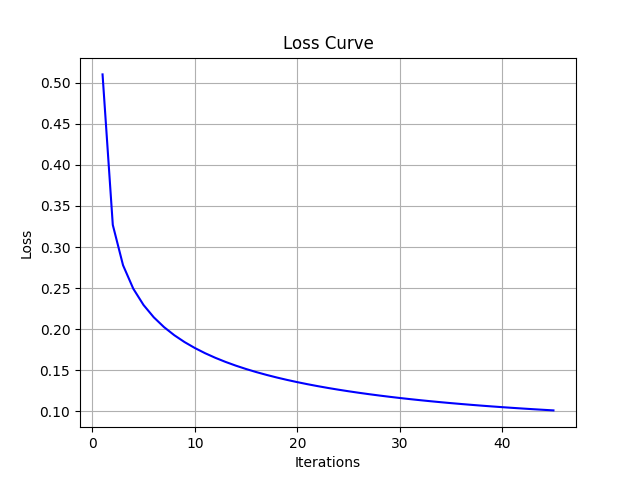
\includegraphics[width=0.5\textwidth]{./result/pretrain1.png}
  \caption{第一轮预训练loss下降曲线}
  \label{fig:example}
\end{figure}

第二步,还是使用1/10的数据和第一步选出的特征在第一步得到的模型的缩减版(删除已经被删除的特征所对应的权值,并按比例减少 bias)进行训练。

这一步是因为使用全部数据进行训练,每个 epoch 所需时间太长,所以先使用较少的数据使 loss 快速下降,然后对所有数据训练时可以减少 epoch 数量,同时还可以优化超参数。loss下降曲线如图2。

\begin{figure}
  \centering
  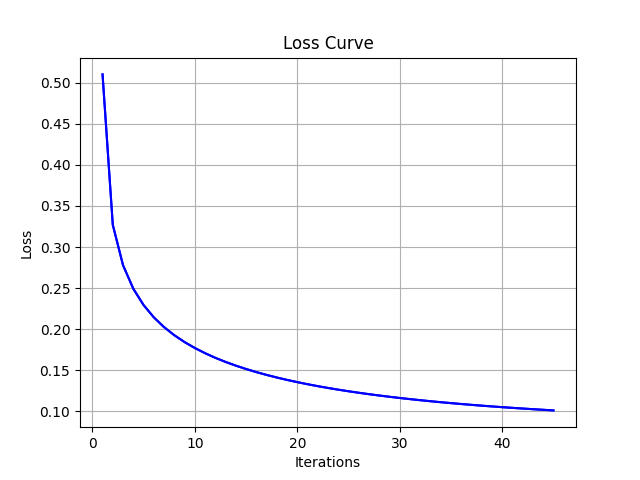
\includegraphics[width=0.5\textwidth]{./result/pretrain2.png}
  \caption{第二轮预训练loss下降曲线(并与第一轮对比)}
  \label{fig:example}
\end{figure}

\section{训练方法}

直接使用全部数据进行参数更新,在每个 epoch 中使用每一条新闻的 feature 对权重进行梯度下降。loss下降曲线如图3。

\begin{figure}
  \centering
  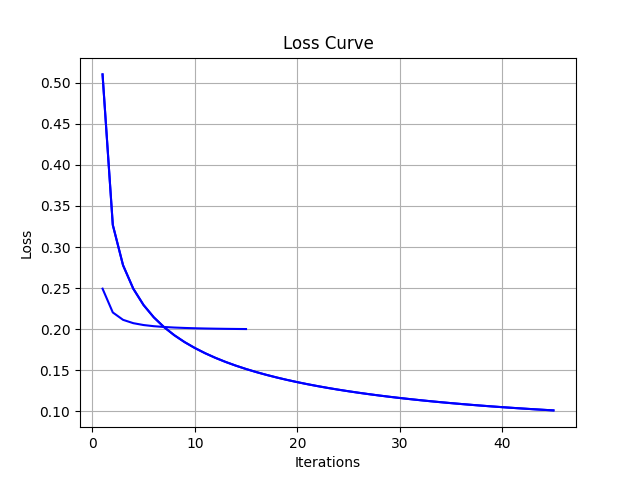
\includegraphics[width=0.5\textwidth]{./result/train.png}
  \caption{最终训练loss下降曲线(并与两轮预训练对比)}
  \label{fig:example}
\end{figure}

\section{实验结果}

当我们使用1028作为第一步特征提取时的每个分类的特征数,4500作为 training 时特征提取最大最终特征数。得到的在训练集上的

准确率约为0.9148

F1 分数为0.9144

在测试集上,先计算模型的混淆矩阵

再计算准确率为0.8975

F1分数为0.8969

和 sklearn.metrics 提供的数值完全相同。

不同特征单词数量得到结果如下表:

\begin{tabular}{|c|c|c|c|c|}
  \hline
  feature\_num & train\_acc & train\_f1 & test\_acc & test\_f1 \\
  \hline
  16 & 0.6308 & 0.6294 & 0.6323 & 0.6309 \\
  64 & 0.8117 & 0.8103 & 0.8104 & 0.8095 \\
  256 & 0.8840 & 0.8831 & 0.8747 & 0.8738 \\
  1100 & 0.9148 & 0.9144 & 0.8975 & 0.8969 \\
  \hline
\end{tabular}

\section{结论}

随着特征数量上升,模型准确性越来越好。

\end{document}
